\documentclass[times, twoside, watermark]{zHenriquesLab-StyleBioRxiv}
\usepackage{booktabs}
\usepackage{lineno}

\begin{document}

\title{Supplemental Material for Quantifying ultra-strong selection in the human genome}
\leadauthor{Dukler}
\shorttitle{ExtRaINSIGHT}
\author[$\ast$, 1]{Noah Dukler}
\author[ $\dagger$, 1]{Yi-Fei Huang}
\author[$\ast$, 2, \Letter]{Adam Siepel}

\affil[$\ast$]{Simons Center for Quantitative Biology, Cold Spring Harbor Laboratory, Cold Spring Harbor, NY}
\affil[$\dagger$]{Department of Biology and Huck Institutes of the Life Sciences, University Park, PA}

%%%%%%%%%%%%%%%%%%%%
%% IMPORTANT: create all labels here with an S prefix so that prettyref can format them correctly in the main doc.
%% Currently implemented prefixes are: Sfig. See the header of the main doc to add more.
%%%%%%%%%%%%%%%%%%%%

\section*{Supplemental Figures}
\begin{figure*}[t]
    \centering
    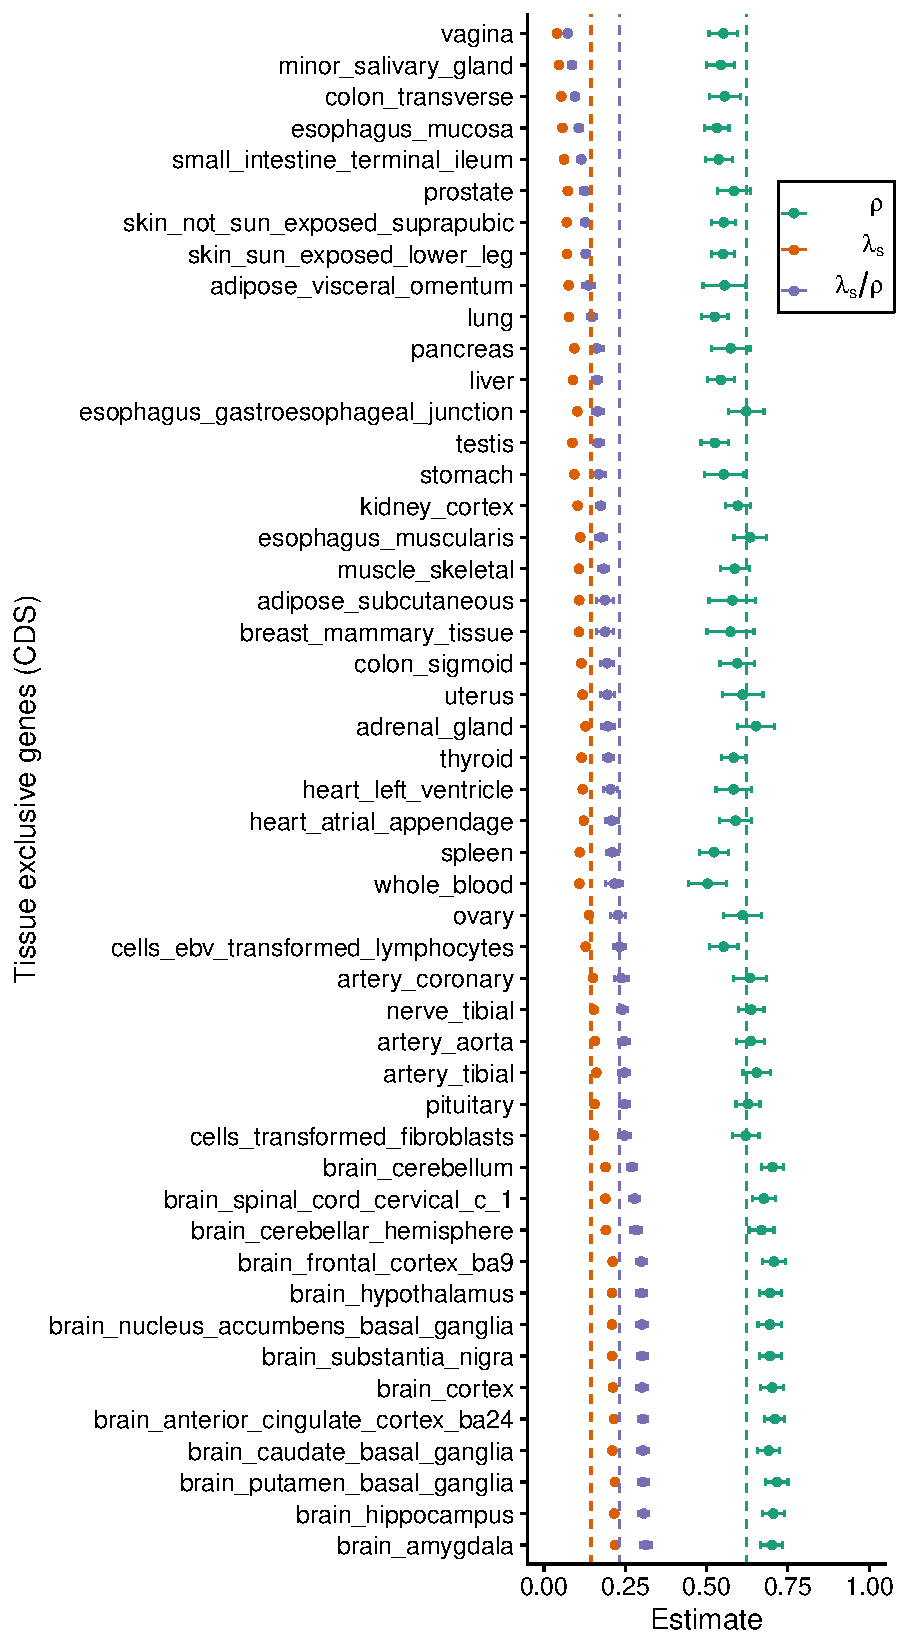
\includegraphics[width=0.6\linewidth]{supplemental_figures/tissue_specificity_cds_ratio.pdf}
    \caption{\textbf{\textbf{ExtRaINSIGHT scores in CDS of tissue-specific genes}}}
    \label{Sfig:tissue_specific_scores}
\end{figure*}

\begin{figure*}
    \centering
    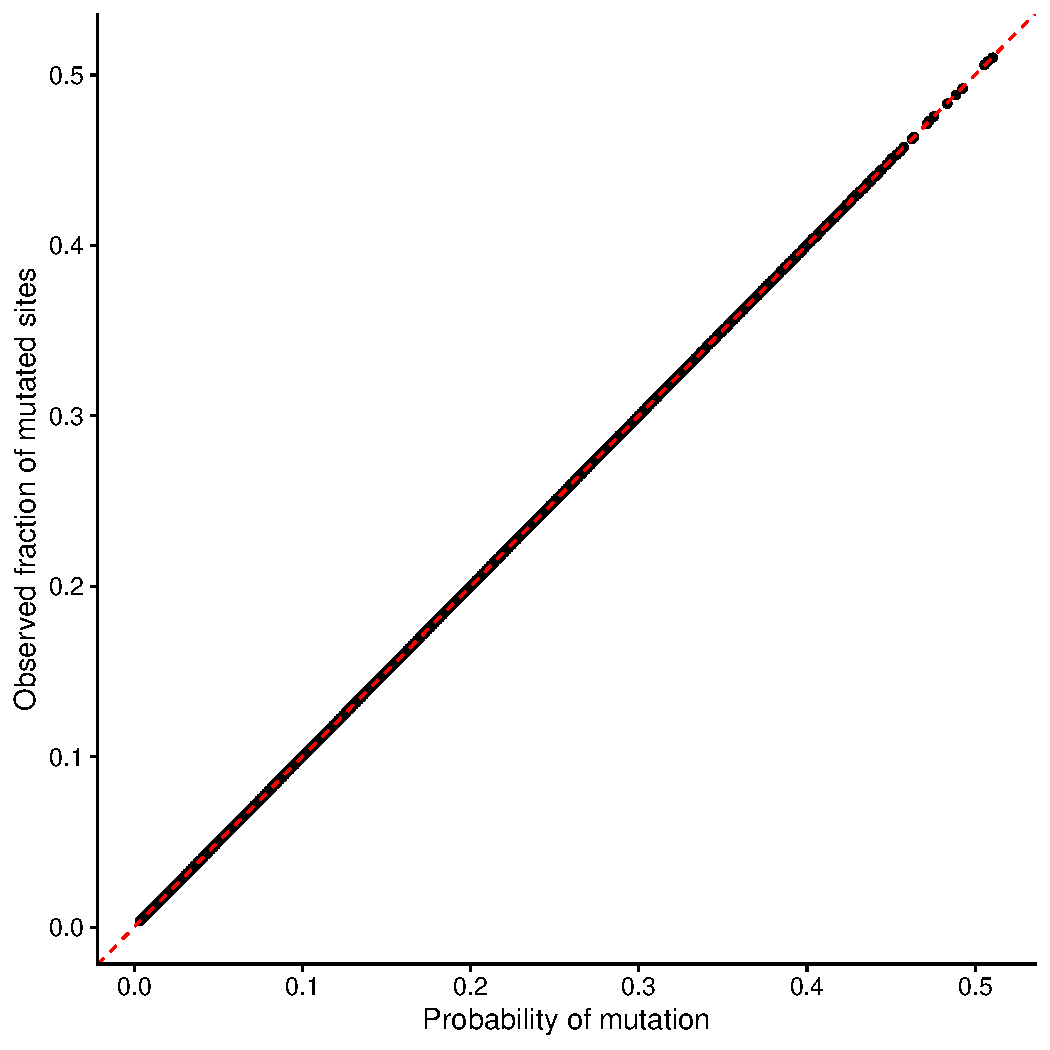
\includegraphics[width = 0.5\linewidth]{supplemental_figures/mutation_model_calibration.pdf}
    \caption{\textbf{The mutation model is globally well calibrated in neutral regions}}
    \label{Sfig:mutation_model_calibration}
\end{figure*}

\end{document}

